% The following is a brief overview on the background and importance of symplectic geometry.

 % Make sure this file exists!

\section{Introduction to Symplectic Geometry}

The goal of this thesis is to present a proof of a Delzant Correspondence for Hamiltonian $\text{SO}(3)$ actions. This introduction answers three fundamental questions:

\begin{enumerate}
    \item What is a meaningful reformulation of classical mechanics?
    \item What is a moment map?
    \item Why is one interested in Delzant's Theorem and its generalizations?
\end{enumerate}

\subsection{Motivation for Symplectic Geometry}

In 15th century CE, Fermat discovered the least path principle for light, which dictates that light will always travel on a path such that its travel time is a local minimum in the space of possible paths. The index of refraction of a material, $\beta \in \mathbb{R}^{+}$, is a scalar quantity which is the factor by which light slows in a material, $v_{\operatorname{eff}} = c/\beta$. Fermat's principle explains Snell's law, which states for two media with indices of refraction $\beta_{1}$ and $\beta_{2}$, a light ray striking the $\beta_{1}$-indexed material at an angle $\theta_{1}$ from the normal will scatter at an angle $\theta_{2}$. The scattering angle $\theta_{2}$ is determined by the three parameters $\beta_{1}$, $\theta_{1}$ and $\beta_{2}$ via $\beta_{1} \sin \theta_{1} = \beta_{2} \sin \theta_{2}$. Snell's law revolutionized the way mechanics was done. \bigskip 

\begin{center}
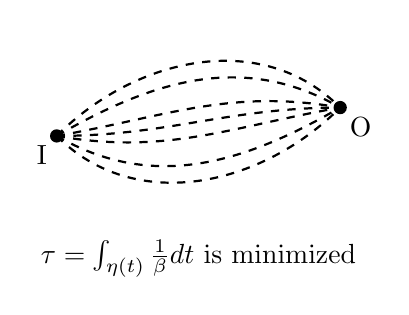
\begin{tikzpicture}[scale=1.2]
    % Define points S and O
    \coordinate (I) at (0,0);
    \coordinate (O) at (3,0.3);
    
    % Draw points S and O
    \fill (I) circle (2pt) node[below left] {I};
    \fill (O) circle (2pt) node[below right] {O};
    
    % Draw multiple paths between S and O
    % Upper paths
    \draw[dashed,thick] (I) to[out=10,in=170] (O);
    \draw[dashed,thick] (I) to[out=30,in=150] (O);
    \draw[dashed,thick] (I) to[out=45,in=135] (O);
    
    % Middle paths
    \draw[dashed,thick] (I) to[out=0,in=180] (O);
    
    % Lower paths
    \draw[dashed,thick] (I) to[out=-10,in=-170] (O);
    \draw[dashed,thick] (I) to[out=-30,in=-150] (O);
    \draw[dashed,thick] (I) to[out=-45,in=-135] (O);
    
    % Add figure label
    \node at (1.5,-1.3) {$\tau = \int_{\eta(t)} \frac{1}{\beta} dt$ is minimized};
\end{tikzpicture}
\end{center}

\noindent This principle was generalized to the Lagrangian Principle, which states that for a mechanical system, described by position $(q^{1}, \dots, q^{n})$ and velocity $(\dot{q}^{1}, \dots, \dot{q}^{n})$, we can construct a scalar function $\mathcal{L}(q^{i}, \dot{q}^{i})$ called the Lagrangian, such that its integral, called the action, is stationary for $\eta(t)$ in the space of possible paths. 

\begin{equation}
\delta S = \delta \left[ \int_{\eta(t)} \mathcal{L} dt \right] = 0
\tag{The Variational Principle}
\label{VariationalCondition}
\end{equation}
\noindent One may show this condition is equivalent to $\mathcal{L}$ satisfying the following differential equation: 

\begin{align}
\frac{\partial \mathcal{L}}{\partial q^{i}} - \frac{d}{dt} \frac{\partial \mathcal{L}}{\partial \dot{q}^{i}} = 0 \text{ for all coordinates } q^{i} 
\tag{The Euler-Lagrange Equations}
\end{align}

\noindent Now, suppose we are given a scalar quantity, $H$ called the Hamilitonian, such that:
\begin{equation}
    \dot{p}_i = -\frac{\partial H}{\partial q^i} 
    \quad \mbox{and} \quad 
    \dot{q}^i = \frac{\partial H}{\partial p_i}
\end{equation}

\noindent Consider the expression:
\begin{equation}
\mathcal{L} = \sum_{i} p_{i} \dot{q}^{i} - H
\label{eq:Hamiliton}
\end{equation}

\noindent Applying the definitions, it follows that:

\begin{align}
\frac{\partial \mathcal{L}}{\partial q_{i}} = -\frac{\partial H}{\partial q_{i}} \text{ and } \frac{\partial \mathcal{L}}{\partial \dot{q}_{i}} = p_{i} \text{ imply } && \frac{\partial \mathcal{L}}{\partial q^{i}} - \frac{d}{dt} \frac{\partial \mathcal{L}}{\partial \dot{q}^{i}} = 0
\tag{A New Formula for $\mathcal{L}$}
\end{align}

\noindent Therefore, \ref{eq:Hamiliton} is the Lagrangian for a mechanical system. The action $S$ for this mechanical system is then written: $S = \int_{t} p_{i} dq^{i} - H dt \label{SymplecticPot}$. 
Symplectic geometry was invented to study the term $\theta = p_{i} dq^{i}$ in the integral of $S$. Namely, the symplectic form, the primary tool of symplectic geometry, is defined to be $\omega = -d \theta$. 

\begin{remark}
From the integral based intuition for $\omega$ - understanding $\omega$ is equivalent to understanding how the integral $S$ behaves
\end{remark}

\noindent \textbf{References: } \textcite{Arnold2010}, \textcite{Terek2020}, \textcite{Feynman:1494701}

\subsection{Delzant's Correspondence Theorem}
In this thesis, we describe how a scalar function generates vector fields One structure that we impose is a Lie group action on our manifold. Now, when a Lie group $G$ acts on a manifold $M$, it establishes an orbit map $\sigma_{p}: G \to M$. This map can be differentiated at the identity of $G$, giving rise to a linear transformation $\left( d \sigma_{p} \right)_{e} \colon \mathfrak{g} \to T_p M$, where $\mathfrak{g}$ is the Lie algebra of $G$. Define the action field corresponding to $X \in \mathfrak{g}$ to be $X^{\#}_{p} = \left( d \sigma_{p} \right)_{e} X$. For each vector field, we ask the question: Does there exist a function which generates this vector field? These functions are known as moment maps and are crucial to the symplectic framework. 

\begin{figure}[htbp]
    \centering
    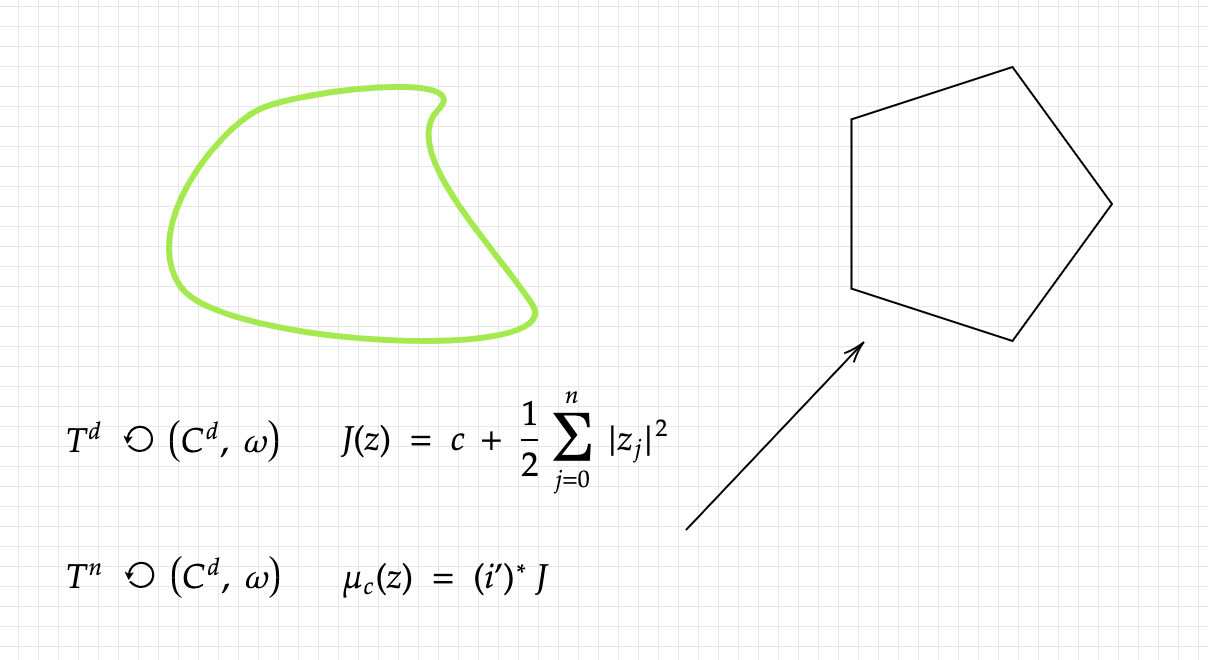
\includegraphics[width=.6\linewidth]{Chapters/Figures/Screenshot 2025-02-05 at 8.59.25 PM.png}
    \caption{Identifying polytopes $\Delta$ as images of moment maps via Delzant's Theorem.}
    \label{fig:delzant_theorem}
\end{figure}

\noindent One classical result in symplectic geometry is Delzant's Correspondence Theorem. It states that there is a one-to-one correspondence between symplectic toric manifolds and Delzant polytopes --- the latter arise as images of moment maps associated with the former. Denote a polytope $\Delta$. Then its corresponding Delzant space is $(X_{\Delta}, \omega)$. Delzant's Theorem is quite interesting because it establishes that the images of momentum maps themselves are geometric objects. Understanding what happens for more general Hamiltonian $G$-spaces (where $G$ is any compact and connected Lie group, not necessarily the torus) is one of the most challenging problems in symplectic geometry. 

\begin{figure}[htbp]
    \centering
    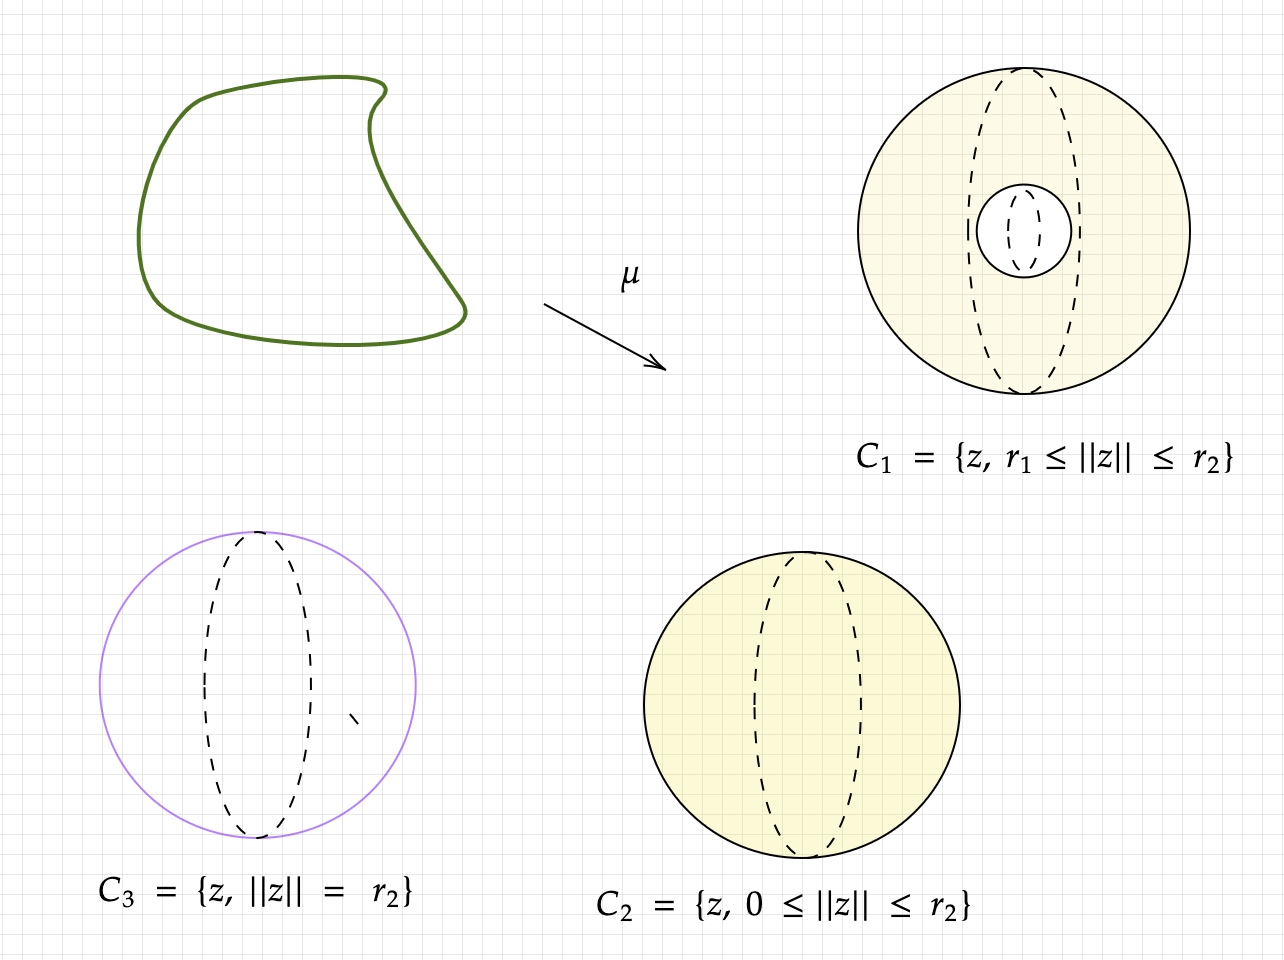
\includegraphics[width=.6\linewidth]{Chapters/Figures/Screenshot 2025-02-06 at 9.44.33 AM.png}
    \caption{Possibilities of nontrivial moment-images when $\text{SO}(3) \circlearrowright M$.}
    \label{fig:so3_moment_images}
\end{figure}

\noindent Now, our investigation starts with the simplest compact and connected non-Abelian group: the special orthogonal group $\text{SO}(3)$. The moment-images for (compact and connected) Hamiltonian $\text{SO}(3)$-spaces, which are necessarily $\text{SO}(3)$-invariant subsets of $\mathfrak{so}(3)^*\cong \mathbb{R}^3$, can then only fall into one among four cases: the origin, a sphere, a closed ball, or a closed hollow ball. It is easy to construct examples showing that all four possibilities do occur, but to which precise extent does this image determine the original space? What is a Delzant correspondence for Hamiltonian $\text{SO}(3)$-spaces, if there is even one at all? \bigskip 

\noindent \textbf{References: } \textcite{AtiyahGS1982}, \textcite{Delzant1988}, \textcite{Blaom1996}

